%%%%%%%%%%%%%%%%%%%%%%%%%%%%%%%%%%%%%%%%%%%%%%%%%%%%%%%%%%%%%%%%%%%%%%%%%%%%%%%%
%2345678901234567890123456789012345678901234567890123456789012345678901234567890
%        1         2         3         4         5         6         7         8

%\documentclass{article}
\documentclass[letterpaper, 10 pt, conference]{ieeeconf}  % Comment this line out
                                                          % if you need a4paper
%\documentclass[a4paper, 10pt, conference]{ieeeconf}      % Use this line for a4
                                                          % paper


\overrideIEEEmargins
% See the \addtolength command later in the file to balance the column lengths
% on the last page of the document

\usepackage[utf8x]{inputenc}
\usepackage{cite}
\usepackage{graphicx}
\graphicspath{{figs/}}
\DeclareGraphicsExtensions{.pdf,.jpg,.png}

\usepackage[draft]{fixme}

\newcommand{\ie}{{\textit{i.e.\ }}}
\newcommand{\cf}{{\textit{cf\ }}}
\newcommand{\eg}{{\textit{e.g.\ }}}


\title{\LARGE \bf
Explicit Knowledge and the Deliberative Layer: Lessons Learned
}

\author{Séverin Lemaignan and Rachid Alami\\
CNRS-LAAS, 7 av. du Colonel Roche, F-31077 Toulouse, France\\
Université de Toulouse, UPS, INSA, INP, ISAE, LAAS, F-31077 Toulouse, France\\
{\tt surname.name@laas.fr}
}

\begin{document}

\maketitle
\thispagestyle{empty}
\pagestyle{empty}


%%%%%%%%%%%%%%%%%%%%%%%%%%%%%%%%%%%%%%%%%%%%%%%%%%%%%%%%%%%%%%%%%%%%%%%%%%%%%%%%
\begin{abstract}

Over the last four years, we have been slowly ramping up explicit knowledge
representation and manipulation in the deliberative and executive layers of our
robots. Ranging from situation assessment to symbolic task planning, from
verbal interaction to event-driven execution control, we have built up a
\emph{knowledge-oriented} architecture which is now used on a daily basis on our
robots.

This article presents our design choices, the articulations between the diverse
deliberative components of the robot, and the strenghts and weaknesses of this
approach. We show that explicit knowledge management is not only a convenient
tool from the software engineering point of view, but also pushes for a
different, more \emph{semantic} way to address the decision-making issue in
autonomous robots.

\end{abstract}


%%%%%%%%%%%%%%%%%%%%%%%%%%%%%%%%%%%%%%%%%%%%%%%%%%%%%%%%%%%%%%%%%%%%%%%%%%%%%%%%
\section{A Knowledge-Oriented Architecture}

\subsection{The LAAS deliberative layer}

We can give a broader look at the knowledge and the streams of knowledge in our
systems.  Based on the experience gained while developing and deploying {\sc
ORO}, our ontology-based knowledge server, we have presented how symbolic
knowledge could be produced from perception and geometric reasoning in modules
like {\sc SPARK}, a grounded, perspective-aware, geometric reasoner. We have
seen how symbolic knowledge could be reused by different control systems and
task planners like {\sc Cram}, {\sc SHARY}, {\sc pyRobots}, the {\sc CLSU
Toolkit} or {\sc HATP} and how they take advantage of semantic abstractions
provided by knowledge base. We have also presented the bidirectional
integration of {\sc Dialogs}, a natural language processor for English, with
the knowledge base.

Altogether, these components compose an architecture that we call
\emph{knowledge-oriented}:

\begin{itemize}
    
    \item{Knowledge is explicitly stored in one central and consistent
    repository of facts, accessible by all modules.} 

    \item{Knowledge is represented in a strict formalism (OWL statements) and
    with a clearly defined vocabulary (stated in the common-sense ontology).}

    \item{The first two points enable both a loosely-coupled architecture where
    modules can very easily be removed or replaced by other ones as long as
    they share the same semantics (modules are defined by the knowledge they
    produce),} 

    \item{and a \emph{symbolic} reactive, event-driven approach to supervision.
    By managing events at the same level as the reasoner, we take full
    advantage of the inference abilities of ORO to trigger events whose
    \texttt{true} conditions can be inferred.} 

    \item{Finally, this architecture allows for the combination of very
    different knowledge modalities in a single homogeneous environment,
    bringing mutual benefits to components. For instance, the dialogue
    processing module can perfectly run without any geometric
    perception, but its disambiguation routines can transparently
    benefit from it when available (since richer symbolic descriptions of
    objects are then available).}

\end{itemize}

This architecture moves away from standard layered approaches. Interactions
between components are mostly bidirectional and, from the software components
point of view, we do not introduce layers of abstraction (we do, however, have
access to the lower level modules of the robot to execute actions, but all
cognition-related modules reside at the same level). This is especially visible
for the dialogue input processing. This component does not simply act as an
alternative perceptual input to the symbolic database, but also actively
queries previously acquired knowledge to disambiguate and validate the newly
created symbolic knowledge.

Our architecture relates but is to be distinguished from \emph{Beliefs,
Desires, Intentions} (BDI) architectures. BDI architectures are primarily
focused on \emph{practical reasoning}, \ie the process of deciding, step by
step, which action to perform to reach a goal (as summarised by
Woolridge~\cite{Woolridge1999}). The management of the interaction between
knowledge (the beliefs) and task and plan representation and execution (the
desires and the intentions) is central, and aims at selecting at each step the
best subgoal. It becomes then an intention that the robot commits to.

This interaction between knowledge and actions is also central to our approach
(as for any cognitive system), but task representation and task execution is
not seen as a monolithic, central function: it is one of the activities of the
robot, actually split between communication components (that can acquire
desires from interaction with agents, amongst other things) and an execution
controller that may decide to take an incoming desire into account to create
its own internal goals. The controller generates and controls intentions from
these goals with the help of a symbolic task planner, that has also direct
access to the knowledge base.

The architecture is not only focused on this workload, and other
activities are conducted without being explicitly considered as desires:
assessment of the situation and the environment, dialogue (including
performative dialogue that can possibly change the internal state of the robot,
but does not lead to the creation of desires,  like question answering or
statement assertion), various background monitoring and recognition tasks, etc.

Regarding the anchoring question, this architecture is bidirectional. The
components we described provide a \textit{bottom-up} grounding process: SPARK
and \textsc{Dialogs} constantly build and push new symbolic contents about the
world to ORO where it becomes accessible to decisional layers. In parallel, ORO
relies on reasoning in a \textit{top-down} way to produce new facts that may
trigger in return physical behaviours. 

We believe that this \emph{knowledge-oriented} approach has a strong potential
not only to enable rich human-robot interaction, but also as a broader approach
to information alignment and fusion in complex robotic systems.  The
versatility of this paradigm could be illustrated by a simple imaginary
scenario with a blind robot and a deaf robot. The blind robot does not see (no
cameras or alike), but someone can verbally describe a scene to it. On the
other hand, the deaf robot has a good vision system, but cannot process verbal
input.  Without any changes to the software architecture that we described,
control modules of both robots could equally perform the same tasks since all
the knowledge is abstracted and centralised (note that to actually implement
this imaginary situation, the blind robot would of course need \textit{a
priori} 3D models of objects talked about to enable planning or pick and place
actions, and the deaf robot would require at least some gesture interpretation
to understand orders).

This architecture may also contribute to bring closer robotics and psychology:
it provides clear entry points to implement some classical psychology tests to
robots. For instance, we presented experiments focused on issues related to
perspective taking. By explicitly enabling independent modeling of the beliefs
of each agent, our architecture is especially well suited to set up cognitive
and psychological experiments that involve a theory of mind, such as
\emph{False-Belief} experiments, as recently presented in~\cite{Warnier2012a}.



\cite{Alami2011}

\begin{figure*}
        \centering
        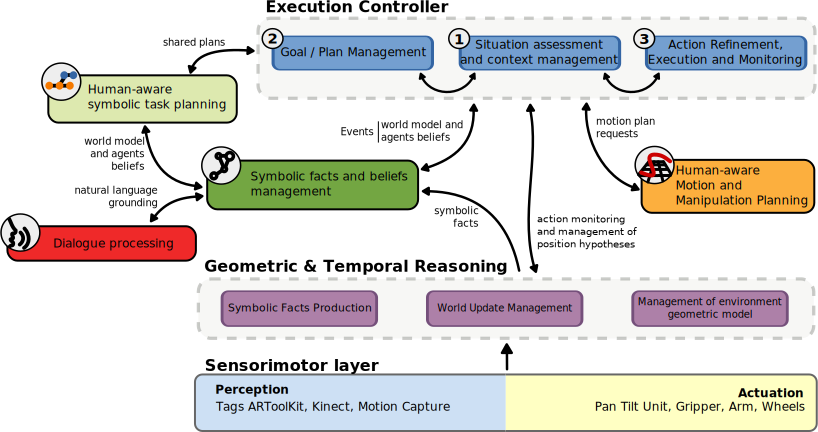
\includegraphics[width=1.7\columnwidth]{archi}
        \caption{Overview of the LAAS deliberative layer.}
        \label{fig|archi}
\end{figure*}

\subsection{Knowledge Model}

\cite{Lemaignan2010}

%%%%%%%%%%%%%%%%%%%%%%%%%%%%%%%%%%%%%%%%%%%%%%%%%%%%%%%%%%%%%%%%%%%%%%%%%%%%%%%%
\section{Situation Assessment}
\label{sect|sit-ass}

\begin{figure}
        \centering
        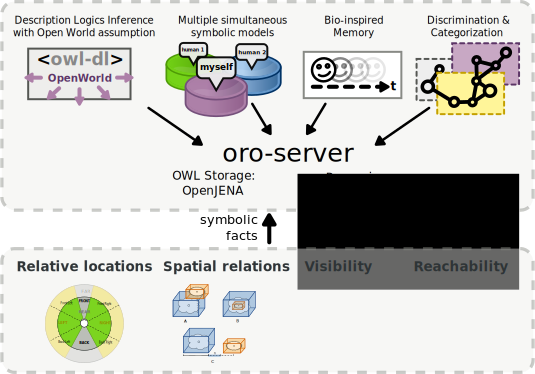
\includegraphics[width=\columnwidth]{spark-oro}
        \caption{Functional overview of knowledge base (\emph{oro-server}, top part) and the geometric situation assessment module (\emph{SPARK}, bottom part)}
        \label{fig|spark-oro}
\end{figure}

\cite{Sisbot2011}

%%%%%%%%%%%%%%%%%%%%%%%%%%%%%%%%%%%%%%%%%%%%%%%%%%%%%%%%%%%%%%%%%%%%%%%%%%%%%%%%
\section{Communication}
\label{sect|com}

\cite{Lemaignan2011a}

\subsection{Disambiguation at semantic level}

\cite{Ros2010b}

\fxnote{Mention failures like 'placeOing'}

\subsection{Multi-modal communication}

%%%%%%%%%%%%%%%%%%%%%%%%%%%%%%%%%%%%%%%%%%%%%%%%%%%%%%%%%%%%%%%%%%%%%%%%%%%%%%%%
\section{Robot Control}
\label{sect|ctrl}

\subsection{Modeling the interaction}

We split the interaction situations stemming from the situation assessment and
communication components in two categories: \emph{desires} and
\emph{experiences}.

Experiences comprise of emotions and questions
\subsection{Task planning}

\cite{Alili2008}

%%%%%%%%%%%%%%%%%%%%%%%%%%%%%%%%%%%%%%%%%%%%%%%%%%%%%%%%%%%%%%%%%%%%%%%%%%%%%%%%
\section{Internal Cognitive Processes}
\label{sect|intern}

\subsection{Theory of Mind}

\cite{Warnier2012a}

\subsection{Working Memory}

%%%%%%%%%%%%%%%%%%%%%%%%%%%%%%%%%%%%%%%%%%%%%%%%%%%%%%%%%%%%%%%%%%%%%%%%%%%%%%%%
\section{Conclusions}
\label{sect|conclusion}

\subsection{The Architect view: loose coupling and modalities merging}

\subsection{The Logician view: the importance of trivial inferences}

\begin{quote}

    Where to find milk? Milk is a subclass of dairy which is itself a subclass
    of a perishable goods. The usual storage place for perishable goods is the
    fridge, so the milk is likely to be found in a fridge.

\end{quote}

This example of reasoning, quoted from Moritz Tenorth, is a good example of
simple yet non-trivial reasoning. As a matter of fact, only very few of such
reasoning cases where positively identified in our scenarii and experiments
(and consequently implemented as rules in ORO).

The design choices of our architecture partially explain that fact: first, the
planning task (which is the prototypical reasoning task) is delegated to a
dedicated, external planner. Then, time is not represented in ORO, and
consequently no temporal reasoning takes place at this level: action
recognition or monitoring are handled by other layers, and the underlying
reasoning tasks are not implemented as explicit symbolic rules in the knowledge
base.

The experiments we have conducted are also likely to have too simplistic
semantics to let complex reasoning needs to emerge. Scenarii with more complex
semantics would be desirable to better stress the expressiveness and inference
abilities provided by description logics.

Is reasoning at the knowledge level immature or even superfluous, then? Not so:
hundreds of trivial (from a human point of view) inferences are continuously
produced by the system (translating inheritance relations, domain/range
constraints, transitivity, etc.) and encode a large amount of common-sense
knowledge that would be tedious, to say the least, to manually assert. These
trivial inferences are all the more important that an expressive knowledge
representation language is used: when a language like OWL allows to directly
represent high-level concepts like partitions, cardinality restrictions,
properties' ranges and domains, it leads to a more implicit (because more
abstract) description of the vocabulary that in turn requires more underlying
reasoning. With the progress in the understanding of the relations between
expressiveness and (tractable) satisfiability, along with the progress of
reasoners, more and more of the inferences do not need to be explicit anymore,
and consequently move behind the scenes.

And we predict that \emph{common-sense encoding} is likely to remain the main
application of reasoning in our robotic architectures, where reasoning related
to decision making mostly happen outside the knowledge representation system.


\subsection{The Cognician view: palpable knowledge and semantic thinking}

The main motive goal was to transform the knowledge in the robot from some ubiquitous,
pervasive, multi-modal and, most importantly, mostly undefined feature of the
system into an observable, quantifiable, manipulable resource, what we could
call a \emph{palpable} feature.

This transformation, both from the technical point of view (the ORO server, the
ontologies, the bindings, etc.), and as a more subtle change in the practises
related to the development of robotic components, is the main contribution of
this thesis.

Knowledge is not an abstract concept anymore: it is a set of statements, in
most cases directly intelligible to the developers, stored in one place. We can
export them, monitor them, review them, question them.

Communication between the robot's module is now conceived in term of what are
the \emph{semantics} of the information flows, instead of a simple
compatibility of interfaces. When defining the frontiers of a robotic
component, we do not think anymore only in term of ``is the interface complete
and self-contained'', but also in term of ``is the semantic complete and
consistent?''. This allow a deeper, more correct modularity: two modules that
share the same, well-defined semantic can be confidently exchanged. When we
remove or disable a component (the dialogue processing, the geometric
reasoning, ...), we know precisely what knowledge will not be available
anymore.

We call this new property of our robot, that allows for both qualitative and
quantitative analysis of the beliefs, its \emph{cognitive observability}.

It is somewhat related to the idea of \emph{cognitive penetrability} introduced
by Pylyshyn~\cite{Pylyshyn1989} in 1989, in the context of the study of
possible strong equivalences between computational models and the
\emph{psychological reality}:

\begin{quote}

    [One of the criterion] relies on the assumption that we can identify
    certain clear cases of phenomenon that should be accounted for at the
    knowledge level, that is, in terms of the representations alone, rather
    than in terms of properties of the cognitive architecture. Phenomena that
    depend in a rational way on subjects' goals, beliefs, and utilities are a
    case in point. For example in psychophysics we assume that if a measure
    (such as a threshold) changes systematically as we change the payoffs (that
    is, the relative cost of errors of commission and of omission), then the
    explanation of that change must be given at the knowledge level -- in terms
    of decision theory -- rather than in terms of properties of sensors or
    other mechanisms that are part of the architecture. In general showing that
    certain empirical phenomena are sensitive to goals and beliefs (or what I
    call \emph{cognitively penetrable}) is prima facie evidence that they
    should not be attributed to properties of the architecture.

\end{quote}

The introduction of an explicit \emph{knowledge level} in our architecture
makes it possible to effectively assess the cognitive penetrability of the
whole robot behaviours (this is however not new, and traditional BDI
architectures would also make this claim).

\section*{Acknowledgment}

This work has been supported by EU FP7 ``SAPHARI'' under grant agreement no. ICT-287513.

\bibliographystyle{IEEEtran}
\bibliography{IEEEabrv,biblio}


\end{document}
